\section{Validierung}

- Fragen vom Anfang erfüllt?\\

- Funktionsweise gegeben?\\
- Gpio Test mit Schaltung
- Spi Kommunitkation. Test mit Oszi (Screenshots)



% Oszi-Bild , wie es aussehen sollte
\begin{figure}[H]
	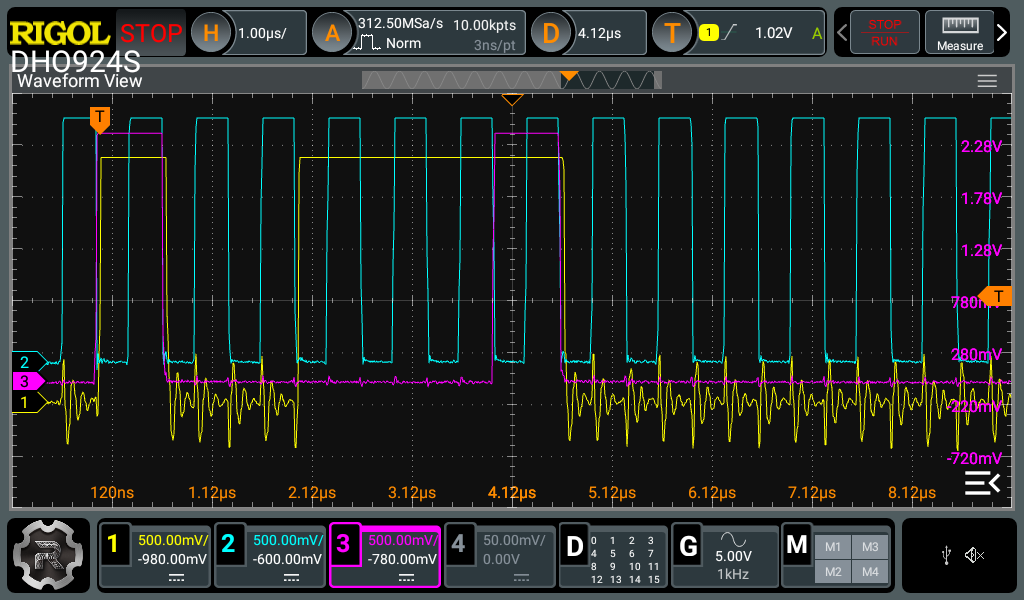
\includegraphics[width=\textwidth]{Pics/oszi_cube_spi_example.png}
	\caption{Screenshot des Osziloskopbildschirms. Dieser zeigt die Wellen für SCK (blau), MOSI (magenta) und MISO (gelb).}
	\label{fig:oszi_cube_spi_example}
\end{figure}

So sollten die Wellen auch mit dem Plattformunabhängigen Code aussehen.

\begin{figure}[H]
	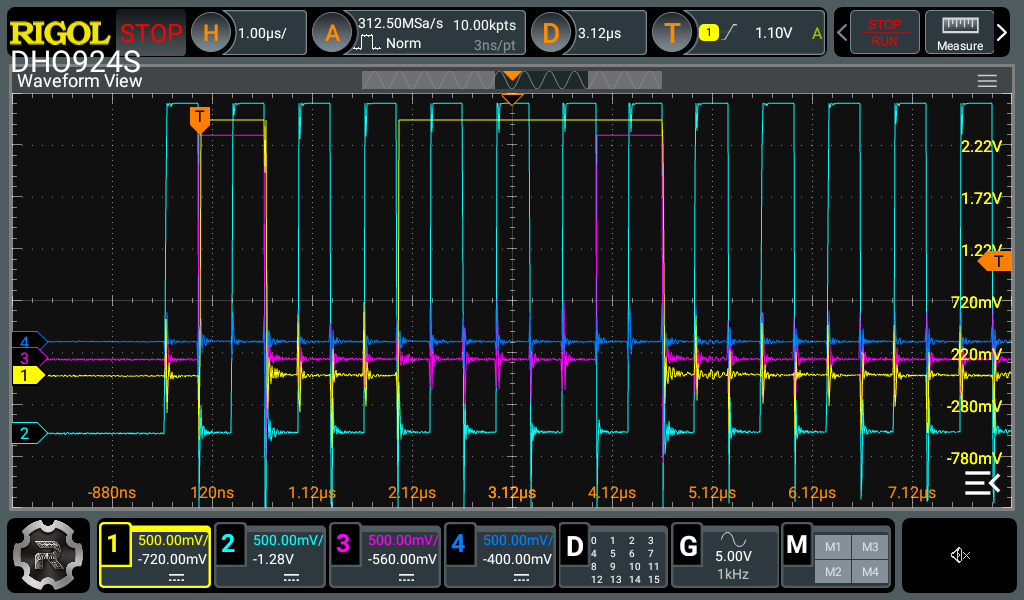
\includegraphics[width=\textwidth]{Pics/spi_signal_test.png}
	\caption{Screenshot einer erfolgreich SPI-Kommunikation, erstellt mit dem Code der HW\_API.}
\end{figure}









































